\documentclass[a4paper, oneside, 10pt]{book}

\usepackage{fancyhdr,verbatim, listings, color} 
\usepackage{shorttoc}
\usepackage[french]{minitoc}
\usepackage[pdftex]{graphicx} 
\usepackage[utf8]{inputenc}
\usepackage[T1]{fontenc}
\usepackage[frenchb]{babel}
\usepackage{amsmath,amssymb,mathrsfs}
\usepackage[french]{varioref}
\usepackage{url}
\usepackage{../nota}
\usepackage{../citation}
%\usepackage{../sommaire}

\graphicspath{%
  {../imgs/}%
  {imgs/}
}

% NOTES
\setlength{\largeurnota}{.8cm}
\newenvironment{attention}{%
  \begin{pictonote}{attention}}{\end{pictonote}}
\newenvironment{note}{%
  \begin{pictonote}{note}}{\end{pictonote}}
\newenvironment{question}{%
  \begin{pictonote}{question}}{\end{pictonote}}

\usepackage[pdftex=true,
    bookmarks         = true,
    bookmarksnumbered = true,
    bookmarks = true, 
    pdfstartview      = FitH,
    bookmarksopen     = true, 
    bookmarksopenlevel = 1, 
    hyperindex        = true,
    colorlinks        = true,
    %urlcolor          = red,
    %pdfborder         = {0 0 0}
    ]{hyperref}

\definecolor{colKeys}{rgb}{0,0,1} 
\definecolor{colIdentifier}{rgb}{0,0,0} 
\definecolor{colComments}{rgb}{0,0.5,1} 
\definecolor{colString}{rgb}{0.6,0.1,0.1} 

\lstset{
float=hbp,
basicstyle=\ttfamily\small,
identifierstyle=\color{colIdentifier},
keywordstyle=\color{colKeys},
stringstyle=\color{colString},
commentstyle=\color{colComments},
language=c++,
columns=flexible,
tabsize=2,
frame=trBL,
frameround=tttt,
extendedchars=true,
showspaces=false,
showstringspaces=false,
numbers=left,
numberstyle=\tiny,
breaklines=true,
breakautoindent=true,
captionpos=b,
commentstyle=\textit
}

\lstnewenvironment{java}{\lstset{language=Java}}{}

%% Define a new 'leo' style for the package that will use a smaller font.
\makeatletter
\def\url@leostyle{%
  \@ifundefined{selectfont}{\def\UrlFont{\sf}}{\def\UrlFont{\small\ttfamily}}}
\makeatother
%% Now actually use the newly defined style.
\urlstyle{leo}

\pagestyle{fancy} 



\hypersetup{
    pdfauthor   = {Clément Badiola, Samuel Da Silva, Alexandre Perrot, Ladislav Marsik, Reda Lyazidi},% 
    pdftitle    = {CP - Rapport de projet},%
    pdfsubject  = {Rapport de projet},% 
    pdfkeywords = {},% 
    pdfcreator  = {PDFLaTeX},% 
    pdfproducer = {PDFLaTeX}} 

\author{Clément~\textsc{Badiola} \and Samuel~\textsc{Da~Silva} \and Reda~\textsc{Lyazidi} \\
\and Ladislav~\textsc{Marsik} \and Alexandre~\textsc{Perrot} \\
  Client : Hugo~\textsc{Balacey}}
\title{Conduite de projet \\ Rapport du projet}
\date{4 novembre 2012}

\begin{document}

\fancyhf{} 
\renewcommand{\chaptermark}[1]{\markboth{#1}{}} 
\renewcommand{\sectionmark}[1]{\markright{\thesection\ #1}} 
\fancyhead[R]{\bfseries\thepage}% Left Even, Right Odd - No de page 
\fancyhead[L]{\bfseries\rightmark} % Left Odd - Titre section 
\renewcommand{\headrulewidth}{0.5pt}% filet en haut de page 
\addtolength{\headheight}{0.5pt} % espace pour le filet 
\renewcommand{\footrulewidth}{0pt} % pas de filet en bas 
\fancypagestyle{plain}{ % pages de tetes de chapitre 
  \fancyhead{} % supprime l’entete 
  \renewcommand{\headrulewidth}{0pt} % et le filet 
}

\fancypagestyle{plain}{
	\fancyhf{}
	\fancyfoot[C]{\thepage}
	\renewcommand{\headrulewidth}{0pt}
	\renewcommand{\footrulewidth}{0pt}}

\dominitoc

\maketitle

\frontmatter

\chapter{Introduction}

Ce document est le rapport d'un projet de conduite de projet effectué par un groupe de 5 étudiants dans le cadre de leur deuxième année de Master.

Le projet concerne blablabla. Il s'agissait de développer des fonctionnalités dans le cadre blablabla et des bonnes pratiques blabla.

\vfill

\textbf{Mots-clés :} conduite de projet, agile, scrum, gestion

\vfill
 %Contexte, problematiques à étudier.

\tableofcontents

\mainmatter

\chapter{Gestion de projet}
\minitoc

\section{Gestion de projet}
%Explication et distribution des roles scrum, vision du projet (objectifs, jalons, utilisateurs visés) et mise en place du backlog, estimations des points.
\subsection{Pré-requis du projet}
%Choix des outils de dév. (codage, versionnage, bug tracking, integration et tests). Choix des techniques d'integration et des conventions de codage.
\section{Déroulement du projet}

Le projet a été rythmé par une succession de 3 Sprints avec chaque semaine des réunions de projet.  


%Description exhaustive du déroulement des sprints : 
% Réunions de planification de sprints (le quoi avec le PO et le comment avec l'équipe de dév.)
% Gestion des risques (bloquages et decisions prises, previsions des risques à venir) 
% Mélée quotidienne (par mails et par entrevues rapides) 
% Montrer la burndownChart 
% Réunion de revue de sprint (avec le PO, c'est un peu la meme que la réunion de planification en fait...)
% Réunion de rétrospective (les points positifs qu'on a pas trop soulevés^^, et les points à améliorer, genre quand quelqu'un que je ne citerais pas faisait des magnifiques rebases qui pourissaient tout le graphe de notre systeme de versionnage =D)
%Description exhaustive du déroulement des sprints : 
% Réunions de planification de sprints (le quoi avec le PO et le comment avec l'équipe de dév.)
% Gestion des risques (bloquages et decisions prises, previsions des risques à venir) 
% Mélée quotidienne (par mails et par entrevues rapides) 
% Montrer la burndownChart 
% Réunion de revue de sprint (avec le PO, c'est un peu la meme que la réunion de planification en fait...)
% Réunion de rétrospective (les points positifs qu'on a pas trop soulevés^^, et les points à améliorer, genre quand quelqu'un que je ne citerais pas faisait des magnifiques rebases qui pourissaient tout le graphe de notre systeme de versionnage =D)
\subsection{Description du déroulement projet}

Dans cette section, nous allons retracer le déroulement du projet au travers de l'analyse des burndown charts de chacun des sprints.

\subsubsection{Sprint 1}

\begin{figure}[h]
\begin{center}
	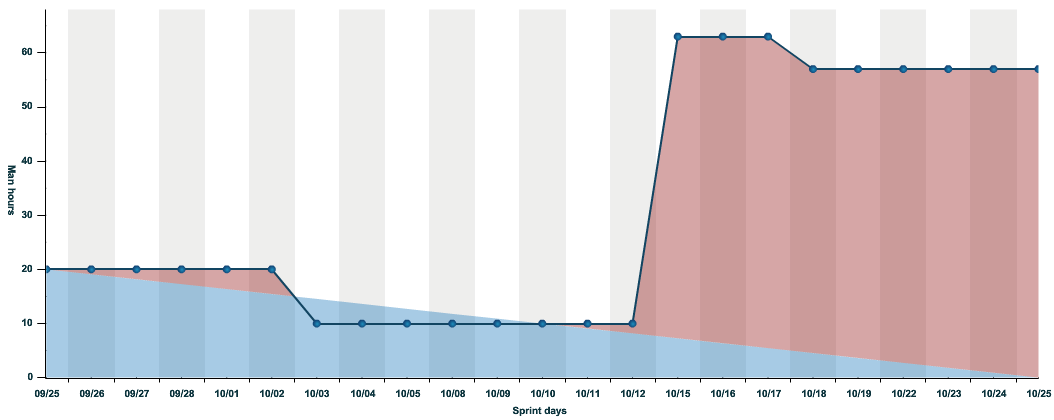
\includegraphics[width=11cm]{burndown-S1.png}
\end{center}
	\caption{Burdown chart du sprint 1}
\end{figure}

L'activité principale de ce premier sprint a été de créer une couche modèle pour notre application. Ceci impliquait de trouver une bibliothèque permettant de lire le format dicom et qui soit compatible avec android. Cette tache a demandé beaucoup d'investissement et de recherche et n'a pu être achevée qu'au sprint suivant. C'est pourquoi on remarque trois plateaux de stagnation. L'augmentation spectaculaire du nombre d'homme-heure restant vers la fin du sprint est du à une mauvaise utilisation de l'outil. En effet, ce sprint nous a introduit à la méthode \emph{scrum} et aux outils associés. De ce fait, notre manque d'assurance et de maîtrise explique les imperfections de ce sprint. Néanmoins, on constate tout de même que des avancées significatives ont pu être réalisées durant ce sprint, la partie modèle étant en majorité achevée lors du passage au deuxième sprint.

\subsubsection{Sprint 2}

\begin{figure}[h]
\begin{center}
	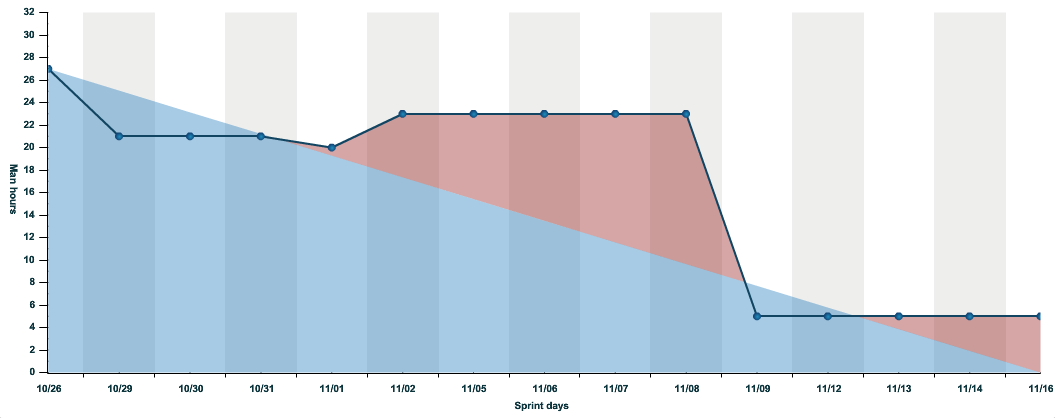
\includegraphics[width=11cm]{burndown-S2.png}
\end{center}
	\caption{Burndown chart du sprint 2}
\end{figure}

Après la prise en main de la méthode \emph{scrum} et des outils au cours du premier sprint, nous avons pu aborder ce deuxième sprint plus en confiance. On constate un bon départ, les tâches les plus faciles ayant été réalisées en premier. Des tâches plus ardues ont ralenti la progression vers le milieu du sprint, mais nous avons su travailler de concert pour surmonter les difficultés et revenir en deçà de la prévision. Les quelques tâches inachevées ont été reportées au dernier sprint. Globalement, ce deuxième sprint est très positif, notre première expérience en \emph{scrum} nous permettant de mieux gérer l'évaluation et la répartition des tâches. Le seul point négatif est la présence de tâches inachevées, c'est pourquoi nous avons décider de revoir notre capacité de travail à la baisse pour le sprint final.

\subsubsection{Sprint 3}

\begin{figure}[h]
\begin{center}
	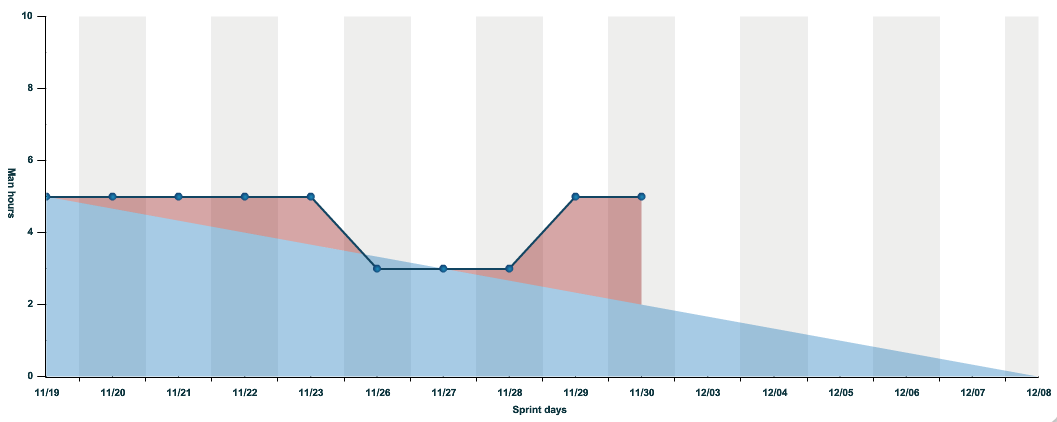
\includegraphics[width=11cm]{burndown-S3.png}
\end{center}
	\caption{Burndown chart du sprint 3}
\end{figure}

Les quelques difficultés rencontrées en début de sprint 3 ont pu être surmontées grâce au concours de toute l'équipe. Les tâches restantes en fin de sprint 2 et les tâches simples du sprint 3 ont été rapidement réalisées. On peut remarquer une augmentation du travail à réaliser. Ceci est du à la modification d'un besoin par le client et son intégration au sprint. Malheureusement, ce sprint n'a pas pu être mené à son terme à cause des impératifs calendaires de rendu.
%partie à modifier en fonction de l'issue du BMI3D
 %THE PARTIE : mise en place du projet (env. de dév., conventions, techniques) et détail du planning. Bien insister sur les screens youkan et github (pour les techniques de merge).
\chapter{Cahier des charges}
\minitoc

Comme nous venons de le voir, notre projet consiste à nous intéresser à la réalisation d'un logiciel d'interaction avec des examens médicaux au format \emph{DICOM} sur tablette tactile \emph{android}. Définissons pour ce programme les objectifs du point de vue non-fonctionnel. Les besoins fonctionnels sont présentés au niveau de la figure \vref{usecase} et détaillés au chapitre \vref{casutilisation}.

\section{Besoins non-fonctionnels}

\subsection{Refactoring}

Le refactoring consiste à retravailler un code source dans le but d'améliorer sa lisibilité et son efficacité, et de simplifier sa maintenance.
L'introduction de nouvelles fonctionnalités induit le besoin de refactoriser souvent le code afin de simplifier
la maintenance et la compréhension.
En plus d'un simple nettoyage, cela nous amène à vérifier que notre architecture répond toujours aux
objectifs fixés.

L'objectif est bien sûr d'obtenir un gain de clarté, de lisibilité, de maintenabilité, et probablement de performances. Nous pouvons ainsi continuer l'ajout de fonctions sur une base saine.

\subsection{Ergonomie}

Le besoin d'ergonomie se fait ressentir car les utilisateurs visés ne sont pas spécialement adeptes des dernières technologies informatiques et ne disposent pas du temps nécessaire au suivi d'une formation préalable à l'utilisation de l'application. L'application doit donc être au possible intuitive et facile à utiliser, malgré les contraintes matérielles. Pour un terminal dont la zone d'affichage est réduite, nous visons donc à maximiser la taille des contrôles tout en minimisant leur interférence sur les zones d'affichage. Cela traduit aussi le besoin de rendre rapide l'accès aux informations des examens.

\subsection{Performance}

L'utilisabilité de l'application passe par ses performances. La puissance de calcul étant limitée sur les terminaux portables, l'enjeu principal est donc de limiter l'usage des ressources tout en maximisant la fluidité de l'interface graphique.

 %Présentation des fonctionnalités demandées.
\chapter{Architecture}
\minitoc

L'architecture constitue un des éléments les plus importants pour le développement d'une bonne application.
Voici les concepts sur lesquels nous nous appuyons pour réaliser une architecture cohérente :  

\begin{itemize}
  \item Garder une architecture la plus simple possible. Chaque classe représente quelque chose de précis.
  \item Ranger les méthodes dans les bonnes classes.
  \item Limiter les attributs des classes afin de limiter les bugs.
  \item Limiter les dépendances externes et au langage. Les langages évoluent vite et il peut être parfois intéressant de pouvoir passer une application sur un autre langage.
\end{itemize}

\section{Diagramme des cas d'utilisation}

Nous avons réalisé un schéma des cas d'utilisations, visible en figure \vref{usecase} afin de synthétiser les besoins de l'utilisateur, pour offrir une vision simplifiée du système. Nous rappellerons brièvement les fonctionnalités par la suite.

\begin{figure}[h]
\begin{center}
    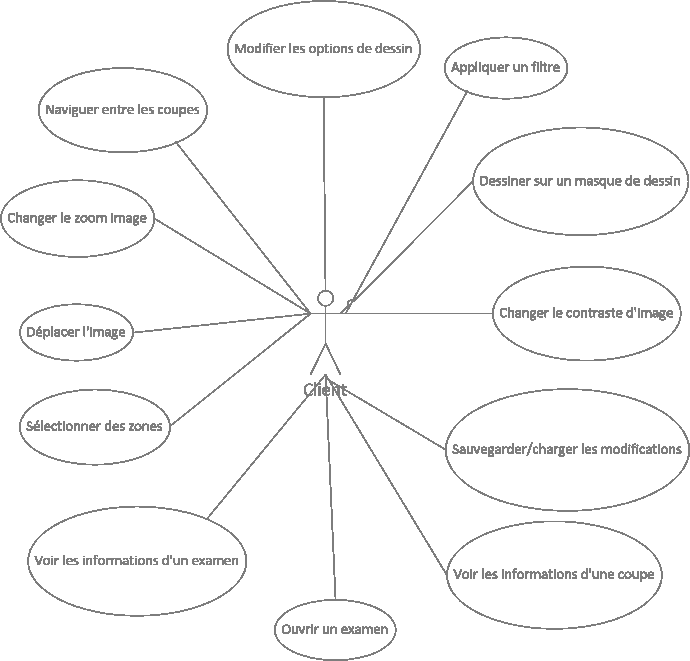
\includegraphics[width=12cm]{diagramme-usecase}
\end{center}
    \caption{Diagramme de cas d'utilisation}
    \label{usecase}                      
\end{figure}

\subsubsection{Ouvrir un examen}

L'utilisateur peut ouvrir un examen stocké sur sa tablette en parcourant l'arborescence de fichiers
et en cliquant sur l'examen choisi.

\subsubsection{Visualiser les informations d'un examen}

Le client peut, n'importe où dans un examen, visualiser les informations associées à cet examen
en cliquant sur un bouton qui déclenchera l'ouverture de la fenêtre d'affichage des informations.
Il pourra y voir des informations sur le patient et sur les conditions d'examen.

\subsubsection{Visualiser les informations d'une coupe}

Le client peut visualiser les informations associées à une coupe
en cliquant sur un bouton qui déclenchera l'ouverture de la fenêtre d'affichage des informations.
Il pourra y voir des informations associées à la coupe affichée à l'écran.

\subsubsection{Naviguer entre les coupes}

Le client peut visualiser les différentes coupes qui composent un examen qu'il a précédemment ouvert
en cliquant sur les boutons associés aux déplacements entre coupes.

\subsubsection{Dessiner des zones sur un masque de dessin}

Le client peut dessiner sur un masque de dessin en superposition avec l'image d'une coupe de l'examen.
Il dispose d'outils de dessin tels que le crayon ou la gomme.

\subsubsection{Modifier les options de dessin}

Le client peut dessiner sur un masque de dessin en variant les effets tels que l'épaisseur du trait
utilisé.

\subsubsection{Modifier le contraste de l'examen}

Le client peut à tout moment changer le contraste (échelle de Hounsfield) des coupes de l'examen ouvert
en utilisant les contrôles associés à cet effet. Il peut modifier la largeur de l'échelle et son centre.
Il peut également choisir un contraste prédéfini parmi une liste de contrastes pour visualiser des éléments
spécifiques tels que les os ou les chairs.

\subsubsection{Se déplacer dans l'image}

Le client peut visualiser différentes portions d'une image en la faisant glisser sur l'écran avec les doigts.

\subsubsection{Changer le niveau de zoom d'une image}

Le client peut modifier le niveau de zoom d'une image en utilisant le contrôle prévu à cet effet.
Il peut augmenter ou diminuer le niveau de zoom.

\subsubsection{Sauvegarder les modifications}

Le client peut enregistrer ses modifications (dessin, contraste par défaut) effectuées sur un examen.

\subsubsection{Restaurer les modifications}

Le client peut charger ses modifications (dessin, contraste par défaut) effectuées auparavant sur un examen.

\subsubsection{Appliquer un filtre}

Le client peut modifier les images d'un examen en appliquant un filtre (tel que le flou gaussien).

\subsubsection{Sélectionner des zones}

Le client peut sélectionner des zones sur une coupe pour appliquer des traitements spécifiquement sur ces
zones.
\section{Les classes}

Les diagrammes de classes de l'architecture du logiciel ont été réalisés à l'aide des logiciel \emph{Architexa} et \emph{UML Lab} intégrés à \emph{Eclipse}. Nous ne parlerons donc que de notre architecture finale, obtenue au fur et à mesure des sprints et refactorings.

Étant donné l'étendue de l'application, nous ne pouvons pas présenter de diagramme UML à la fois complet et lisible dans ce rapport. Commençons donc par obtenir une vue d'ensemble du logiciel à l'aide du diagramme en couches visible en figure \vref{layered-packages}. En bleu, les packages de transformation des données. En vert, les packages utilitaires. En rouge, le cœur de l'application, qui inclut dans des sous-packages le modèle des données, la gestion de cache et les classes d'interface graphique. Les flèches, plus ou moins épaisses, indiquent une dépendance plus ou moins forte d'un package à un autre.
On remarque bien que le package diams constitue le cœur de l'application.
Les packages utilitaires peuvent être changés sans problèmes, car ils ne dépendant pas d'autres packages.
Le package pixelmed constitue une bibliothèque de traitement de fichiers Dicom dont le cœur d'application dépend.
L'enjeu majeur a donc été de rendre l'architecture du cœur d'application la plus flexible possible pour limiter
l'effort requis en cas de changement de bibliothèques.


\begin{figure}[h]
\begin{center}
    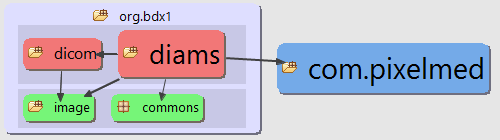
\includegraphics[width=11cm]{diagramme-couche}
\end{center}
    \caption{Diagramme en couches de l'application}
    \label{layered-packages}
\end{figure}

\subsection{Le modèle d'examen}

Voyons maintenant le diagramme des classes du modèle, en figure \vref{classes-model}.
En bleu, les classes utilitaires, en vert le modèle qui représente un examen et les données associées, et en
orange les éléments qui permettent de faire le lien entre le modèle et la bibliothèque d'extraction des images \emph{Pixelmed}.

La classe \verb+DefaultModelFactory+ permet d'interagir depuis l'extérieur avec le modèle d'un examen sans dépendre des autres classes.
La classe \verb+Examen+ est le composant principal qui permet de gérer les autres éléments du modèle.
Un ensemble d'interfaces permet de faciliter des modifications ultérieures sur le modèle.

Notez que la classe orange \verb+LisaImageAdapter+ est le seul élément de dépendance avec la bibliothèque externe \emph{Pixelmed}. Nous avons donc minimisé l'impact que peut créer le passage de \emph{Pixelmed} à un autre outil.


\begin{figure}[h]
\begin{center}
    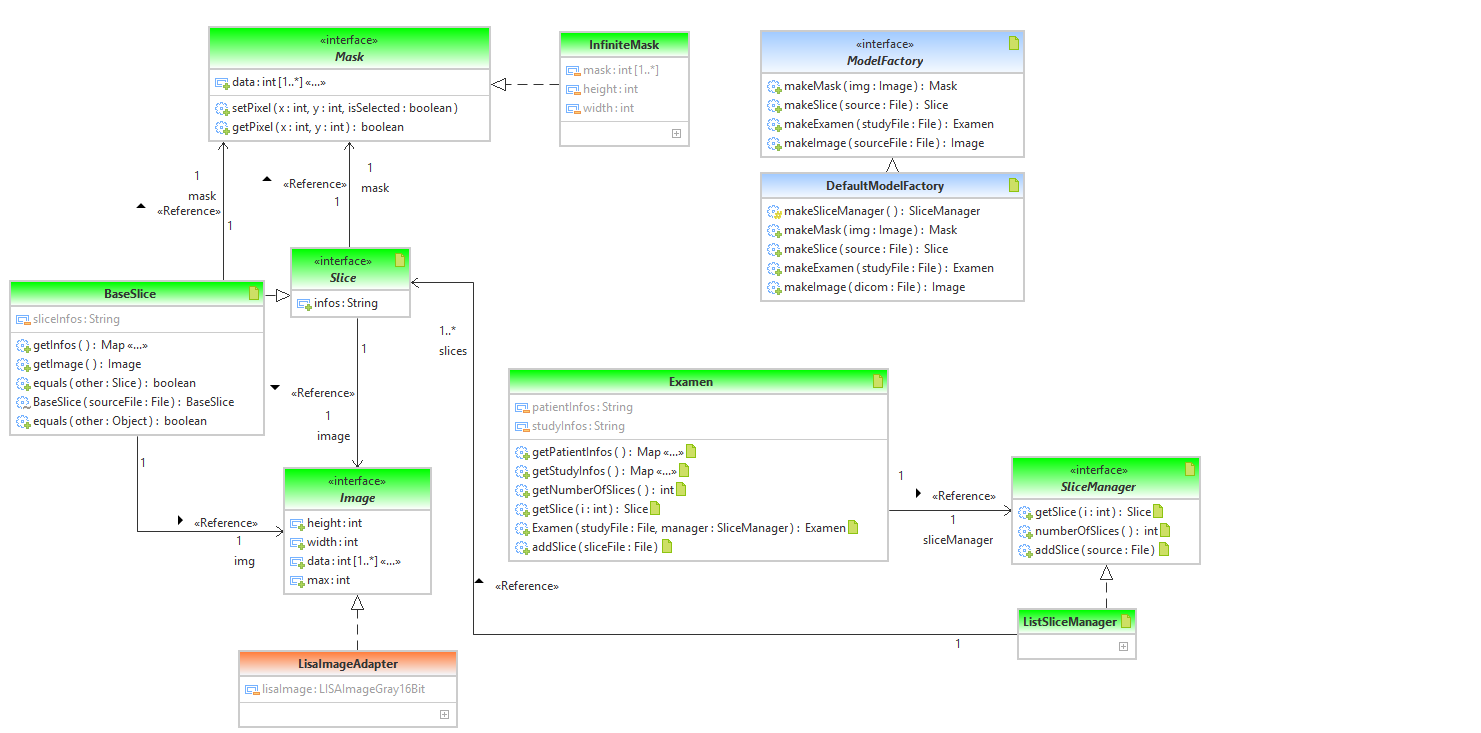
\includegraphics[width=11cm]{diagramme-classes-model}
\end{center}
    \caption{Diagramme de classes du modèle de l'application}
    \label{classes-model}
\end{figure}

\subsection{L'interface graphique}

Nous nous intéressons maintenant au diagramme des classes simplifié de la partie graphique, visible en figure \vref{classes-diams}. En bleu, les classes d'interface graphique. En orange, les classes d'interaction avec les fichiers et en vert la classe d'interaction avec le modèle.

La classe \verb+FileBrowserActivity+ permet, à l'ouverture de l'application, de sélectionner et d'ouvrir un examen parmi une arborescence de fichiers. Les classes \verb+ImageActivity+ et \verb+InfoDisplayActivity+ permettent de visualiser les composants de l'examen choisi et d'interagir avec.
La classe \verb+DicomDirFileHandler+ gère les traitements des fichiers lors de la navigation dans l'arborescence des fichiers.

On note que les dépendances entre l'interface graphique et les données sont limitées à deux classes. Nous avons minimisé l'impact d'un changement de bibliothèque d'interface graphique à ces deux classes.

\begin{figure}[h]
\begin{center}
    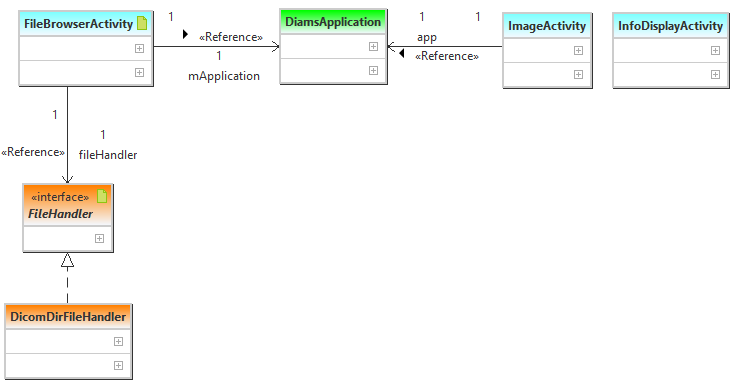
\includegraphics[width=11cm]{diagramme-classes-diams}
\end{center}
    \caption{Diagramme de classes de l'interface graphique de l'application}
    \label{classes-diams}
\end{figure}

\subsection{Le système de cache}

Le développement d'une application mobile entraine des contraintes dues au matériel. La puissance du processeur et la quantité de mémoire vive sont limitées. Notre application devant gérer un grand nombre d'images, nous avons implémenté un système de cache afin de limiter l'occupation mémoire à un instant t, sans pour autant entraver les actions de l'utilisateur par de longs temps de chargement.

Afin que notre couche modèle puisse être réutilisée dans un contexte n'entrainant pas l'utilisation d'un cache, nous avons fait attention à séparer les classes responsables de ce cache des autres classes modèles. Cette problématique nous a tout d'abord conduits à séparer la gestion des coupes de l'Examen proprement dit à travers l'interface \verb+SliceManager+. Nous avons ensuite pu réaliser l'implémentation du cache indépendamment du modèle. La bibliothèque \emph{android} contenant déjà un système de cache, nous avons décidé de l'utiliser pour implémenter \verb+SliceManager+. De cette façon, une seule classe de notre système de cache dépend d'\emph{android}. Enfin, nous utilisons une nouvelle \verb+ModelFactory+ héritant de \verb+DefaultModelFactory+ afin de faire la liaison entre le modèle et le cache.

\begin{figure}[h]
\begin{center}
	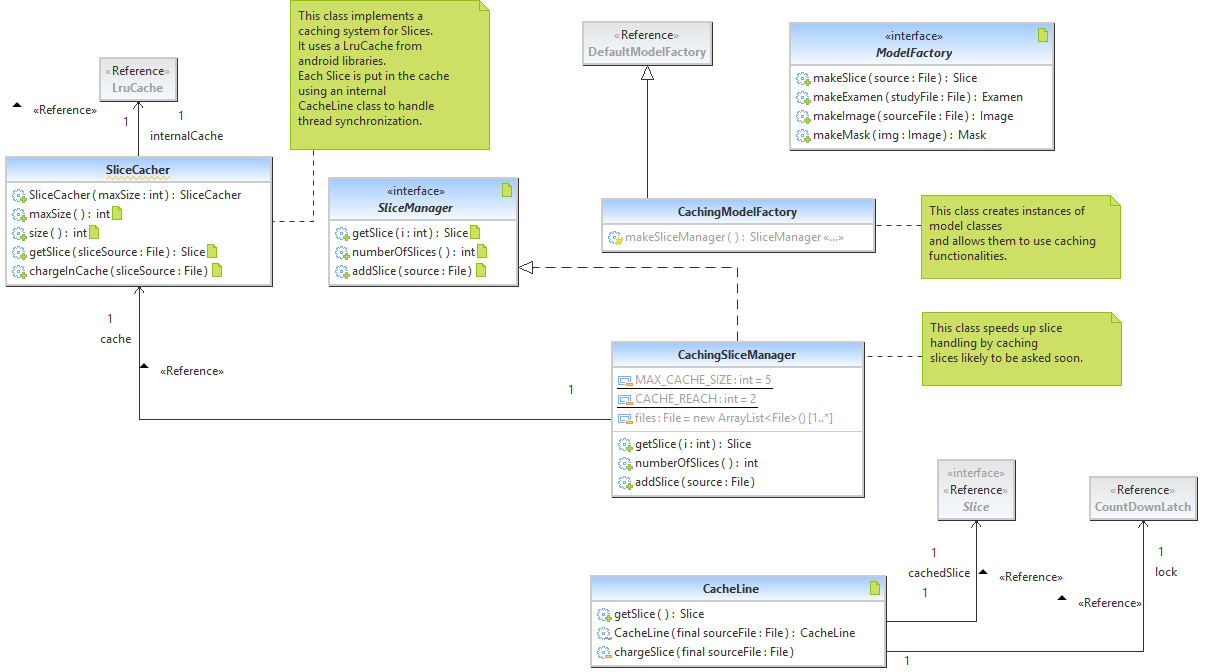
\includegraphics[width=11cm]{diagramme-classes-cache}
\end{center}
	\caption{Diagramme de classes du système de cache}
	\label{classes-cache}
\end{figure}

 %Présentation cas d'utilisation, architecture générale, archi. d'un package...
\chapter{Travail}
\minitoc

\section{Travail}
\subsection{L'explorateur de fichiers}

\begin{figure}[h]
\begin{center}
    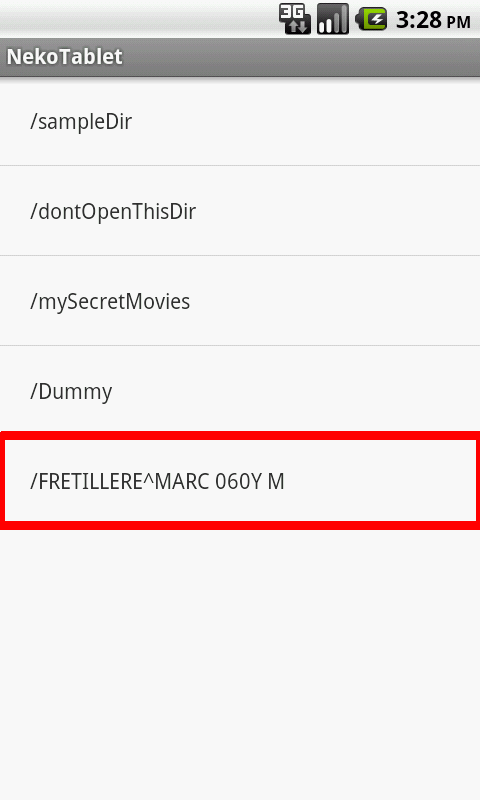
\includegraphics[width=12cm]{file-browser}
\end{center}
    \caption{Capture d'écran de l'explorateur de fichiers}
    \label{fichiers}                      
\end{figure}

L'ouverture de l'application conduit sur l'écran d'exploration des fichiers, visible en figure \vref{fichiers}.
Nous distinguons les dossiers normaux des dossiers \emph{DICOM}. Sur la figure \vref{fichiers}, on peut voir qu'un dossier a été entouré en rouge : il s'agit d'un exemple de dossier \emph{DICOM}. Ces derniers représentent un examen et contiennent les fichiers qui constituent les données de l'examen. Le nom du dossier \emph{DICOM} est masqué à l'utilisateur, qui voit à la place le nom, le prénom, le genre et l'âge du patient associé à l'examen.
Un clic sur un dossier quelconque place la vue à l'intérieur du dossier. On peut revenir dans le dossier parent par autre clic. Un clic sur un dossier \emph{DICOM} déclenche l'ouverture de l'examen et l'utilisateur passe alors sur l'affichage présenté dans le chapitre suivant.
\subsection{L'interaction avec un examen}

Après avoir ouvert un examen, l'utilisateur se retrouve face à la fenêtre principale de l'application. Cette fenêtre présente la première tranche de l'examen ouvert. L'utilisateur peut la déplacer en utilisant l'écran tactile. Il peut aussi régler le niveau de zoom grâce au curseur prévu à cet effet. 
Le menu de l'application permet d'accéder aux informations de l'examen et de la coupe courante. Enfin, l'utilisateur peut basculer d'une coupe à une autre avec les boutons situés en haut de la fenêtre.\\

\begin{figure}[h]
\begin{center}
	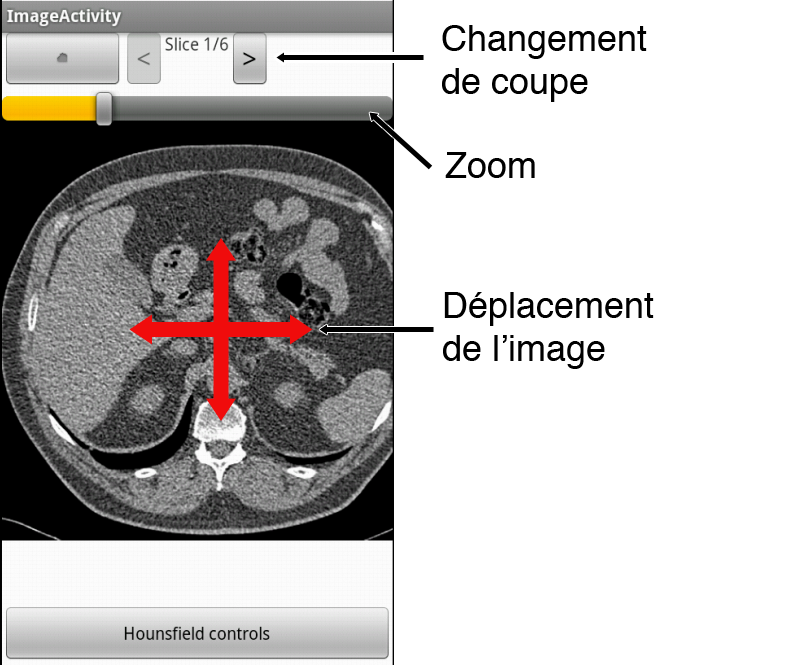
\includegraphics[width=11cm]{diams-capture-1.png}
\end{center}
	\caption{Fenêtre principale en mode déplacement}
\end{figure}

En bas de la fenêtre se trouve un menu coulissant permettant de gérer l'affichage de l'image à l'aide de l'échelle de Hounsfield. Deux curseurs permettent de régler la position et la taille de la fenêtre de valeurs à afficher. De plus, un menu déroulant permet de sélectionner des valeurs de contraste correspondant à des usages courants. L'affichage de l'image est alors mis à jour en temps réel.\\

L'utilisateur peut passer du mode déplacement de l'image au mode dessin sur le masque grâce à un bouton situé en haut de la fenêtre. Dans ce second mode, il est possible de réaliser des sélections de zone avec un crayon ou d'effacer des tracés existants. Une option permet de contrôler la largeur du tracé.\\

\begin{figure}[h]
\begin{center}
	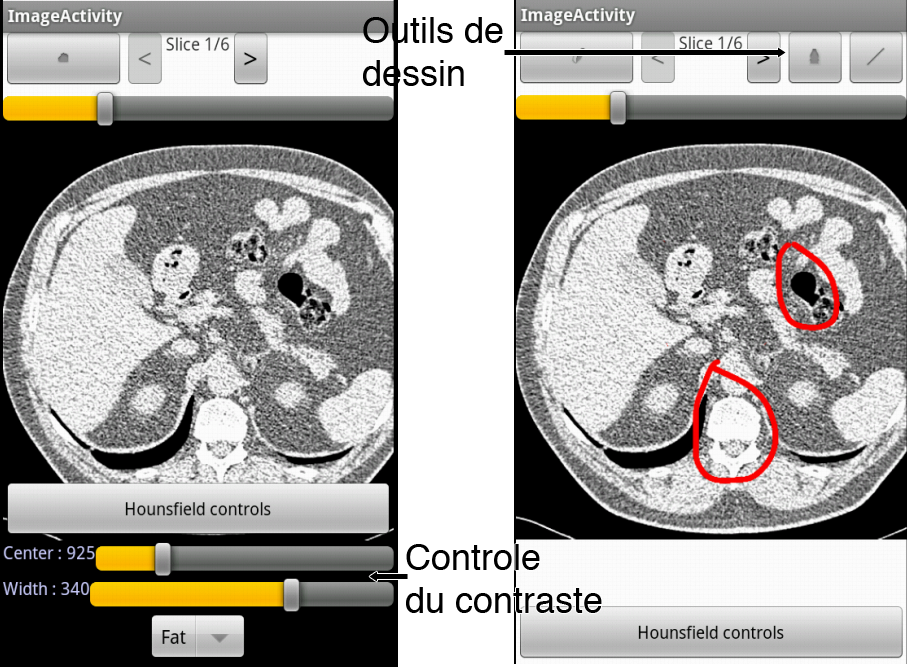
\includegraphics[width=11cm]{diams-capture-2.png}
\end{center}
	\caption{Réglages de contraste à gauche et mode dessin à droite}
\end{figure}

\section{Tests}

Afin de garantir la fiabilité de nos livrable, nous réalisons une série de tests unitaires et de tests fonctionnels. Les tests unitaires nous permettent de nous assurer du bon fonctionnement de certaines parties déterminées du logiciel. 

\subsection{Test 1}
Nous réalisons un ensemble de tests de blablabla. afin de blabla. %Pas sûr qu'on garde cette partie
\chapter{Bilan}
\minitoc

\section{Bilan}

En conclusion, nous pouvons dire que le bilan général est plutôt bon. Nous avons globalement satisfait les besoins client tout en réalisant nos objectifs initiaux en terme de blablabla.

Au niveau de l'architecture, les méthodes sont restées simples, ce qui limite selon nous les sources de bugs. Nous limitons les dépendances avec les bibliothèques Java. L'application est donc plus maintenable et évolutive.

\subsection{Échecs}

Malgré ce bilan positif, nous déplorons blablabla.


\section{Si c'était à refaire…}

Si c'était à refaire, nous aborderions le problème différemment. En incluant nos connaissances en gestion de projets, nous pourrions aborder les problèmes liés à la complexification des phases d'intégration. En connaissant les patterns aux sein d'une équipe, nous aurions pu mesurer les effets de leur utilisation dans le cadre d'un projet utilisant les
méthodes agiles, comme l'\emph{XP} par exemple.

%%\section{Perspectives}
%Voir si on met quelque chose dedans ou non.

 %Ai-je besoin d'expliquer cette partie ? ;)

\appendix
\backmatter
\listoffigures

%\tableofcontents

\newpage
\pagestyle{empty}

Rapport de projet de conduite de projet.\\
DIAMS or Neko tablet.\\
Master 2, 2012

\vfill

Les sources de ce rapport sont disponibles librement sur \url{https://github.com/mr-nours/rapport-cp}.

\end{document}
